% !TEX encoding = UTF-8 Unicode
% !TEX root = thesis.tex

\chapter{Kinesic Signal Prediction \textbf{(Proposed)}}
\label{chapter:prediction}
In this chapter we propose an approach to model kinesic signals in social communication based on a large scale database collected in the Panoptic Studio. Drawing an analogy from telecommunications, social communication can be considered as a process of exchanging messages among people, as senders and receivers, as shown in Figure~\ref{fig:kinesicflow}. The transmitted messages in social communication convey individual's thoughts, emotions, and intentions, which cannot be conveyed by verbal language. Consider a sender sending an internal message to a receiver. The messages originated from the sender's mind are emitted through various channels of signals. The conversion from the internal messages to the emitted social signals inside a sender can be considered as an ``encoding" stage. The converted signals are exposed through display ports of the sender such as voice, facial expressions, and body motions. The signals from the sender are then received by a receiver. The receiver first senses the transmitted signals by body ``sensors" such as eyes and ears. These sensed data is further processed by the receiver's perception system to reason about higher level semantic meanings of the data. For example, kinesic signals are sensed by visual sensors (eyes) as a form of stereo videos, and 3D structures of other people, as well as locations of 3D anatomical landmarks, are inferred. To this end, the signals are interpreted as messages conveying the sender's thoughts.  These processed of a receiver can be considered as a ``decoding" process. 

What we can explicitly measure in this social communication flow is the signals exposed by a sender. In prior work, these signals are observed and manually hand-coded by human annotators into discrete events and categories; otherwise, limited parts in a relatively simple social setup are measured by a few sensors (e.g., face landmarks by a couple of cameras)~\cite{harrigan2013methodology, dael2015measuring}. Our method using the Panoptic Studio allows us to measure kinesic signals of a large group of interacting people at high resolution from full body parts (face, hand, and body). However, it is still unclear how these signals are used to convey information for social communication. These signals exist in a continuous high dimensional space, and a subtle change of the signals can transmit a completely different meaning. Modeling such signals requires analyzing the subtlety embedded in the signals, and, thus, prior work that categorizes them into discrete hand-crafted codes cannot satisfy this requirement. Importantly, we have no way to objectively measure or represent internal messages before the encoding stage by a sender and interpretation of a receiver after the decoding. Manually coding the conveyed messages of the signals means projecting the original high dimensional signals into low dimensional space by a manually defined mapping function, which can cause a severe data distortion and bias. 

In this thesis proposal, we propose an approach to objectively model kinesic communication by continuously predicting an individual's signals responding to the signals from others in a social situation. In our approach, we consider the encoder and decoder of an individual as a single unit as shown in Figure~\ref{fig:senderreceiver}. Our model is defined upon measurable signal inputs and outputs, and we do not explicitly represent or annotate an individual's internal status. By quantifying the prediction performance of the model, we can also evaluate the level of understanding of the proposed model about kinesic communication. 

\begin{figure}[t]
	\centering
	\includegraphics[width=0.6\textwidth]{figures/kinesicmodel}
	\caption{We model each individual's kinesic communication system as a whole single unit. Our model takes signals by others as input, and produces signals of the target individual as output. The goal of our approach is to build a model that understands the flow of kinesic communication. } 
	\label{fig:senderreceiver}
\end{figure}

Conceptually, our approach is similar to a screening test to diagnose autism spectrum disorder, the Rapid Autism Behavior Checklist~\cite{krug1980behavior, mathys2013beyond}. In the protocol, an examiner initiates several predefined activities with a patient, and analyzes the behavior of the patient. Autism spectrum disorder is diagnosed by observing the reactions of the patient and comparing them to that of average people. Similar to our model, social communication ability of the patient is evaluated by the observing the response signals of the patient given a transmitted input signals. 

We use a Deep Neural Network (DNN) to model kinesic communication of humans, and it is trained by our large scale database. The objective of our approach is to build a model to predict instantaneous kinesic signals of an individual given the received signals as input. Various resolution of signals can be considered as the input and output of the model. For example, the model can take full body anatomical landmarks of other people and produce full body response motion of the target individual. In this thesis proposal, we consider a simpler case where the target person's gaze direction is predicted by taking body motions from other people as input. This task enables us to study what type of body motion can be related to the attention of another person in a social situation. The trained model can be considered as a chatbot communicating with humans using kinesic signals. 

Our approach can also be used to evaluate the bandwidth of information conveyed by each body part in kinesic communication. It is widely accepted by social psychologists that much of the emotional meaning is expressed via nonverbal signals \cite{Mehrabian67, Mehrabian81, Birdwhistell70, Moore13}. In related work, researchers try to measure the importance between verbal and nonverbal signal channels (e.g., it is accepted that emotional signals are transmitted by vocal (38 percent), facial expression (55 percent), and verbally (7 percent)~\cite{Mehrabian67, Mehrabian81}). Putting aside that how accurately these percentages are quantified, there is no such literature that tries to measure influence of each body part in kinesic communication. For example, which part is more important between hand motion and facial expression in social communication? Can social communication be affected if some channels of the signals are missing? For example, the bandwidth of transmittable kinesic signals among a face-to-face conversation, a video call, and a phone call should be different, but how can we quantify their differences in term of the relation between the level of available kinesic signals and their influence causing changes in kinesic communication? In building an artificial agent or robot, which type of signals should be measured and emitted by the agent to genuinely communicate with humans? All of these questions are hard to be answered by prior nonverbal communication studies. In this thesis proposal, we propose a way to computationally measure the influence of each body part in social communication. This is performed by quantifying the accuracy of prediction performance of our model by excluding each body signal one-by-one. A preliminary result quantifying influence of each body part related to getting a gaze attention of others is shown in this thesis proposal.  

%As a final goal of our thesis, we try to quantify the influence of each body signal in a social communication task. For example, we measure how important hand gestures are  compared to leg motions in a social communication. We perform the experiment by comparing the prediction performance with and without each signal. In this thesis proposal, we present an influence map of each body part in a gaze prediction task. In all the experiments, a triadic social situation is assumed and the haggling sequences are used for training and testing. 

%In the process of exchanging messages for social communication, it is expected that data loss at each stage may occur. For example, during the process of encoding as a sender, we sometimes experience that our speech or body languages do no fully convey our thoughts. While the signal is transmitted to the receiver, the amount of information may decrease by noise, far distance, and occlusions. The decoding stage by the receiver also may lose the original information by misleading the meaning of sender's messages due to personal and cultural differences. Theses data loss is more severe in non face-to-face communication cases. For example, entire nonverbal signal is missing when people communicate via text messages, and body language is missing in a phone call. A video call also may lose entire signals from lower body or maybe from full body except faces. Any physical disability of senders or receivers also causes data loss of social signals. However, few research has been performed to know how the missing signals affect social interactions. In other words, we rarely know the relative importance of each signals in communications (e.g., How important facial expression is compared to hand gestures). Knowing this knowledge can play an important role not only to understand social communication of people, but also to build virtual agents and robots that socially communicate with humans. 


%In this thesis, we present a framework to model kinesic signals as a way to computationally understand a nonverbal communication of interacting people. In our framework, we train a model to predict a target person's responding kinesic signals by taking kinesic signals of other people as input. Conceptually, the objective of our method is to build a model that can perform a social interaction by receiving and transmitting kinesic signals similar to an individual. The performance of the model can be quantified by comparing the output with ground truth data which is measured from the target person. Various types and combinations of input and output can be considered in defining the model. As an initial task in this thesis proposal, we consider a gaze prediction task of the target person given various combinations of kinesic signals of other people who the target person interacts with. 

%As a major advantage, our method does not require to represent the semantic meaning of a kinesic signal. In most previous work, the mapping between the measured signals and their semantic meanings (e.g., emotions) need to be manually annotated to explicitly regress the encoder and decoder described in the Figure~\ref{fig:kinesicflow2}. However, this process requires the human annotators to map the continuous signal in a high dimensional space to a discrete quantized annotation space, which is subject to bias. More importantly, the manually defined annotations cannot fully express the entire subtlety of the original kinesic signals. In contrast, our method avoids such issue by regressing a encoder and a decoder of an individual as a whole as shown in Figure~\ref{fig:kinesicflow2}, rather than explicitly modeling each of them. Since our model uses measurable kinesic signals as input and output, it has a potential to understand the subtle difference in kinesic signals. We use our dataset to train the model. 

%
%social interactions we use various measured signals by our system including 3D facial landmarks, 3D body landmarks, and 3D hand landmarks. As a way to quantify the relation between social signal and social interaction, we present a novel framework based on predicting output social signals given input signals using Deep Neural Network models. The core advantage of our method is that we do not need to annotate any ``meaning" of each social signals. For example, most of prior work try to annotate the semantic meaning of nonverbal signals, by defining a few categories with quantified levels as annotations. However, since the originals signals are defined in high dimensions and continuous domains, a large amount of important meaning of social signals are missing, putting aside the fact that social signals cannot be objectively annotated. In contrast, our method only use social signals as input and output of the model, and these signals are objectively measurable. 

\begin{figure}
	\centering
	\includegraphics[width=\textwidth]{figures/ssp_notation3}
	\caption{Locations and orientations of an interacting group can be represented by different coordinate systems. (a) Locations and orientations in a world coordinate, (b) Locations and orientations in a person centric coordinate by person $\mathbf{P}_1$, (c) A location of $\mathbf{P}_1$  in a normalized coordinate by a pair of people $\mathbf{P}_2$ and $\mathbf{P}_3$, (d) An orientation of $\mathbf{P}_1$ in a normalized coordinate by a pair of people  $\mathbf{P}_2$ and $\mathbf{P}_3$. } 
	\label{fig:ssp_notation1}
\end{figure}

\section{Notations}

In this section, we formally define the notations of our kinesic signal prediction model, as well as its inputs and outputs. A function $\operatorname{F_i}(\cdot)$  regresses a kinesic signal processing model of the $i$-th person, $\mathbf{P}_i$. It takes the kinesic signals $\mathbf{I}_i$ received by the $i$-th person (from others and oneself) as input, and produces the kinesic signals $\mathbf{O}_i$ emitted by the person as output:
\begin{align}
\mathbf{O}_i=\operatorname{F_i}\left( \mathbf{I}_i \right).
\end{align}

The kinesic signal prediction function can be defined upon various input and output domains, with different level of temporal and spatial resolutions. Input and output signals of the person $\mathbf{P}_i$ at a time instance $t$ is denoted as $\mathbf{I}_i (t)$ and $\mathbf{O}_i (t)$, and we use $\mathbf{I}_i (t_s:t_e)$ and $\mathbf{O}_i (t_s:t_e)$ to represent a series of signals in a range of time from $t_s$ to $t_e$. The input and output can be defined by a set of kinesic signals, and may contain body location $\mathbf{x}_i$, body orientation $\phi_i$, face orientation $\theta_i$, body landmarks $\mathbf{B}_i$\footnote{We use the term ``body" landmark to refer to the landmarks from torso, arms, and legs detected by human body pose detectors~\cite{Belagiannis2014, wei2016convolutional} in computer vision community. It does not contain faces and hands.}, face landmarks $\mathbf{F}_i$, and  hand landmarks $\mathbf{H}_i$. $\mathbf{I}$ contains a combination of these signals received by the target person, and $\mathbf{O}$ contains a combination of social signals emitted by the target person. As an example:
\begin{gather}
\mathbf{I}_1 ( t_s:t) =  \{  \mathbf{x}_1,  \mathbf{x}_2, \mathbf{x}_3,   \theta_2, \theta_3,   \mathbf{F}_2, \mathbf{F}_3,   \mathbf{B}_2, \mathbf{B}_3,   \mathbf{H}_2, \mathbf{H}_3  \}\\
\mathbf{O}_1 (t) =   \{    \theta_1 \}, 
\end{gather}
where each element of $\mathbf{I}_1 ( t_s:t) $ is defined over a time range $t_s:t$ and $\mathbf{O}_1 (t) $  is defined at single time $t$. In this example, the function $\mathbf{O}_1(t) = \operatorname{F}_1 \left( \mathbf{I}_1  ( t_s:t) \right)$ takes a time series of signals from multiple people including the signals from oneself (location $\mathbf{x}_1$) as input, and produces the face orientation of the person at $t$ as a predicted output signal. Intuitively, this function predicts the gaze direction of person $\mathbf{P}_{i}$ at time $t$, by considering a range of kinesic signals up to now. 

The detailed representation of each signal is explained below. 

\noindent \textbf{Location}:	
The location of the $i$-th person is denoted as $\mathbf{x}_i  \in \mathbb{R}^3$, and we use the neck landmark (which is the root of the body skeleton) as the representative location of the individual. The locations at a range of times are denoted by $\mathbf{x}_i(t_s:t) \in \mathbb{R}^{3 \times (t-t_s+1)}$, and it is a vector concatenation of all the locations in the range of time. 

The location of a person can be represented in a person-centric coordinate of a reference person, as shown in Figure~\ref{fig:ssp_notation1} (b). $\mathbf{x}_i^j$ denotes the location of $i$-th person in the person-centric coordinate of $j$-th person. The person-centric coordinate system defined by the $j$-th person can be computed by a corresponding rotation matrix $\mathbf{R}_j$ and $\mathbf{x}_j$:
\begin{align}
	\mathbf{x}_i^j(t)  = \mathbf{R}_j ( \mathbf{x}_i - \mathbf{x}_j).
\end{align}
Note that $\mathbf{x}_i^i$ means its own person centric coordinate system and always becomes the origin. \\

\noindent \textbf{Location in A Normalized-by-A-Pair Coordinate: } 
A coordinate system can be also defined by a pair of people, rather than a single person. In this representation, we ignore y-axis and only consider 2D locations, assuming a view from the top. In this representation, a selected pair of people are located in the origin and a fixed position with a unit distance from the origin respectively. We use $(1,0)$ for the position of the second person of the pair. The objective of this coordinate is to normalize the scale of the formations by the distance of the selected pair, to focus on the shape information only. $\mathbf{x}_i^{j,k}$ represents the location of the $i$-th person in this normalized coordinate defined by locations of a pair of people, $\mathbf{x}_j$ and $\mathbf{x}_k$. A similarity transformation $S(\mathbf{x}_j, \mathbf{x}_k)$ is defined such that it transforms $\mathbf{x}_j$ to $\mathbf{x}_j^{j,k}=(0,0)$, and $\mathbf{x}_k$ to $\mathbf{x}_k^{j,k} = (1,0)$. The similarity function is applied to $\mathbf{x}_i$ to compute $\mathbf{x}_i^{j,k}$ \\

\noindent \textbf{Orientations}: Orientation is represented only w.r.t. $Y$ axis using a single scalar angle value, similar to the method of \cite{mnih2012conditional, Fragkiadaki_2015_ICCV}. Orientation can be defined by either face (denoted by $\phi$) or body (denoted by $\theta$), and only face orientation is explained here. The facial orientation of $i$-th person $\theta_i(t) \in \mathbb{S}$ is computed by projecting the normal vector of the face on XZ plane and computing the counter-clockwise angle from positive X axis, as shown in Figure~\ref{fig:ssp_notation1} (a). From this orientation, we can deterministically compute a rotation matrix $\mathbf{R}_i(t)$ w.r.t. $Y$ axis, which transforms the world coordinate to a person-centric view. We also consider the concatenation of orientations as $\theta_i(t_s:t) \in \mathbb{S}^{t- t_s + 1}$, and its differential, $\Delta \theta_i(t) = \theta_i(t+1) - \theta_i(t) \in \mathbb{S}$.

The orientation can be also represented in a person-centric coordination system. The facial orientation of $i$-th person in a person centric coordinate defined by the $j$-person is denoted as $\theta_i^j$. Because the orientation is defined as a scalar value w.r.t. Y axis, an orientation in a person-centric coordinate can be simply computed as $\theta_i^j = \theta_i - \theta_j$. See the Figure~\ref{fig:ssp_notation1} (b).\\

\noindent \textbf{Orientation in A Normalized-by-A-Pair Coordinate:} Assuming a triadic interaction, we normalize the orientation of a target person by other two selected people, such that the orientation value becomes $0$ when the target person faces a ``right" person, and $1$ when the person faces the other person (the ``left" person). The ``left" and ``right" are defined in the target person's view point, that is by comparing x-axis in the person centric coordinate defined by the target person. The normalized orientation by a pair $\mathbf{P}_2$ and $\mathbf{P}_3$  (assuming the person $\mathbf{P}_2$ is on the left side than $\mathbf{P}_3$ as shown in Figure~\ref{fig:ssp_notation1} (d)) is denoted as $\hat{\theta}_1^{2,3}$, and represented as, 
\begin{align}
\hat{\theta}_1^{2,3} = \frac{\angle \mathbf{g}_1\mathbf{x}_1\mathbf{x}_3}{\angle \mathbf{x}_2\mathbf{x}_1\mathbf{x}_3},
\end{align}
where $\mathbf{g}_1$ represents the head point of the unit vector representing the normal (gaze) direction of $\mathbf{P}_1$. See the Figure~\ref{fig:ssp_notation1} (d). Intuitively, this coordinate system enables that the gaze direction of the target person becomes independent from the world coordinate and the relative orientation of the group.   \\

\noindent \textbf{Body Joint Landmarks: } 
In this thesis, an anatomical body joint at a time $t$ is always represented in a local coordinate system with a fixed skeleton hierarchy. To represent the local coordinate for each joint, we use the relative directional unit vector from a parent joint to a child joint. Each $k$-th body landmark of person $\mathbf{P}_i$ at $t$ in this local coordinate is denoted as $\mathbf{b}_i(k, t)$ and represented as:
\begin{equation}
\mathbf{b}_i(k, t) = \frac{\gamma_i(k, t)  -  \gamma_i ({p(k)}, t)} {|| \gamma_i (k, t)  -  \gamma_i (p(k),t)  ||_2}
\end{equation}
where $\gamma_i (k,t) \in \mathbb{R}^3$ represents the same landmark location in the person-centric coordinate, and $p(k)$ is the index of the parent landmark of the $k$-th joint. Thus, $\mathbf{b}_i(k,t)$ is a unit vector representing the bone direction by canceling out bone length of the person. We also consider a row vector concatenating all joints, $\mathbf{B}_i(t) = \mathbf{b}_i(2:N_j, t)$ (from joint $2$ to $N_j=17$). We ignore the first joint here because it is the root location and already defined by $\mathbf{x}_i$. 
%$\{ b_i^p(t) \}_{N_b} \textrm{, where } j_i^p \in \mathbb{R}^3$

%
%\noindent \textbf{Face Landmarks: } 
%%$\{ f_i^p(t) \}_{N_f} \textrm{, where } f_i^p \in \mathbb{R}^3$
%%53 facial landmarks are generated by the system. To reduce the dimension, we run PCA, and reduce the dimension to 20 variables, $ \eta_i(t) \in \mathbb{R}^{20}$. This particular dimension is chosen to maintain XX percents of the variation in the face. 
%
%\noindent \textbf{Hand Landmarks: } 
%%$\{ h_i^p(t) \}_{N_h} \textrm{, where } h_i^p \in \mathbb{R}^3$
%
%\begin{figure}
%	\centering
%	\includegraphics[width=0.5\textwidth]{figures/ssp_nomalized_gaze}
%	\caption{Orientation in a normalized-by-a-pair coordinate} 
%	\label{fig:ssp_ssp_normalized_gaze}
%\end{figure}

%
%
%We consider a point representing a person's location and its orientation. The point is defined by top of the nose landmark location, and the orientation is defined by the face normal direction, where face normal is computed by the cross product of the line segments of face landmarks as shown in Figure XX. $\mathbf{x}_i(t) \in \mathbb{R}^3$ represents the  location in the world coordinate of subject $i$ at time $t$. And $\mathbf{x}_i(1:t) \in \mathbb{R}^{3 \times t}$ is a concatenated vector of root locations from time $1$ to $t$ of subject $i$. The differential of the location, $\Delta \mathbf{x}_i(t) = \mathbf{x}_i(t+1) - \mathbf{x}_i(t) \in \mathbb{R}^3$, represents location changes in subsequent frames at world coordinate. We represent orientation using a single scalar angle values w.r.t. Y axis, similar to ~\cite{mnih2012conditional, Fragkiadaki_2015_ICCV}. The orientation $\theta_i(t) \in \mathbb{S}$ is computed by projecting the normal vector on XZ plane and measure the counter-clockwise angle from positive X axis. Note that we can deterministically compute rotation matrix $R(\theta)$ w.r.t. y axis from the orientation, which is the rotation from world to person-centric coordinate system.  We also consider a concatenation of the orientations as $\theta_i(1:t) \in \mathbb{S}^{t}$ and also consider its differential 	$\Delta \theta_i(t) = \theta_i(t+1) - \theta_i(t) \in \mathbb{S}$.
%
%We consider the locations in a person centric coordinate system, defined by a person's view point. The $i$-th subject's location changes in $j$-th person centric coordinate system is represented by:
%\begin{equation}
%\mathbf{x}^{j}_i(t) = \mathbf{R}_j\left(\theta(t) \right) \left( \mathbf{x}_i(t) - \mathbf{x}_j(t)  \right) ) + \mathbf{x}_j(t)
%\end{equation}
%
%Using this notation, we can compute the location at $t+1$ in the  person centric coordinate of $t$ of the same person $i$.
%\begin{equation}
%\mathbf{x}^{i}_i(t) = \mathbf{R}_j\left(\theta(t) \right) \left( \mathbf{x}_i(t+1) - \mathbf{x}_i(t)  \right) ) + \mathbf{x}_i(t)
%\end{equation}
%And thus, the differential of root in person centric coordinate system is represented by 
%
%\begin{gather}	
%\Delta \mathbf{x}^{i}_i(t) = \mathbf{R}_j\left(\theta(t) \right) \left( \mathbf{x}_i(t+1) - \mathbf{x}_i(t)  \right) ) \\ \nonumber
%=  \mathbf{R}_j\left(\theta(t) \right) \Delta \mathbf{x}_i(t)  
%\end{gather}
%
%Note that$\Delta \theta_i(t) = \Delta \theta^j_i(t)$, and orientation changes in a person-centric is the same as  changes in world coordinate (since the values is a scalar). 
%
%
%\textbf{Body skeletons}:  Body joint landmarks are considered in person-centric coordinate system by canceling out global translation and orientations.  Each $j$-th joint is represented by the relative unit direct w.r.t. the parent joint:
%
%\begin{equation}
%\gamma_j(i) = j_{i} (t)  -  j_{p(i)} (t) / | j_{i} (t)  -  j_{p(i)} (t)  |,
%\end{equation}
%where $j$ represents location in person-centric coordinate and $gamma_j(i)$ represents our the relative representation w.r.t its parent $p(i)$. We found this representation after canceling out global orientation to make data more coherent. 
%
%\textbf{Face landmark}: As output of our system, 53 landmarks $\{f\}_1^{53}$ are generated to represent a face at a time. To reduce the dimension we run PCA after subtracting the mean of the face, and reduce the dimension to XX, $ \eta \in \mathbb{R}^{20}$. This particular dimension is chosen to have 95 percent of the original variation. 
%
%\textbf{Face and body connection}: Instead of letting face to have full degree of freedom is his location and orientation, we connect face to body using an extra connection between face and body. For the purpose, we introduce an additional connection between head top to the face center (nose top), treating it as other body joints. Since this joint should be rigidly moved with head top and neck joint ideally, we don't need additional rotation parameters for the face. 

%
%
%\section{Negotiation Dataset}
%We present a new game to simulate a haggling among two sellers and a buyer. Two sellers are promoting their own competitive product, e.g., an apple vs chocolates, for selling, and a buyer makes the decision which product he/she chooses to buy between the two. They are given a minute for the haggling, and the seller who successfully sells his/her product is awarded \$5. 

%\subsection{Triadic Negotiation Dataset}
%
%We design a negotiation game to evoke natural nonverbal communications among people. A game is played by three participants, two sellers and a buyer for 1 minute, and the buyer must chose a buyer within the time. We specifically choose a triadic situation, because it contains more diverse and interesting social behaviors (turn taking, gaze following, and formation changes) than other commonly studied dyadic scenes~\cite{rehg2013decoding, lucas2016trust, nojavanasghari2016emoreact}. More importantly we choose a free-standing scenarios (compared to commonly chosen a table-setup) without having any restriction in body motion or appearance other than game rule. To promote a motivation for winning the game, incentives are awarded to the sellers chosen by the buyer. We believe this designed (but natural) setup can induce people to focus more on the social signals currently emerged among them rather than long-term histories, which allow us to approximate the Equation~\ref{equation:F_ours}.

\begin{figure}
	\centering       
	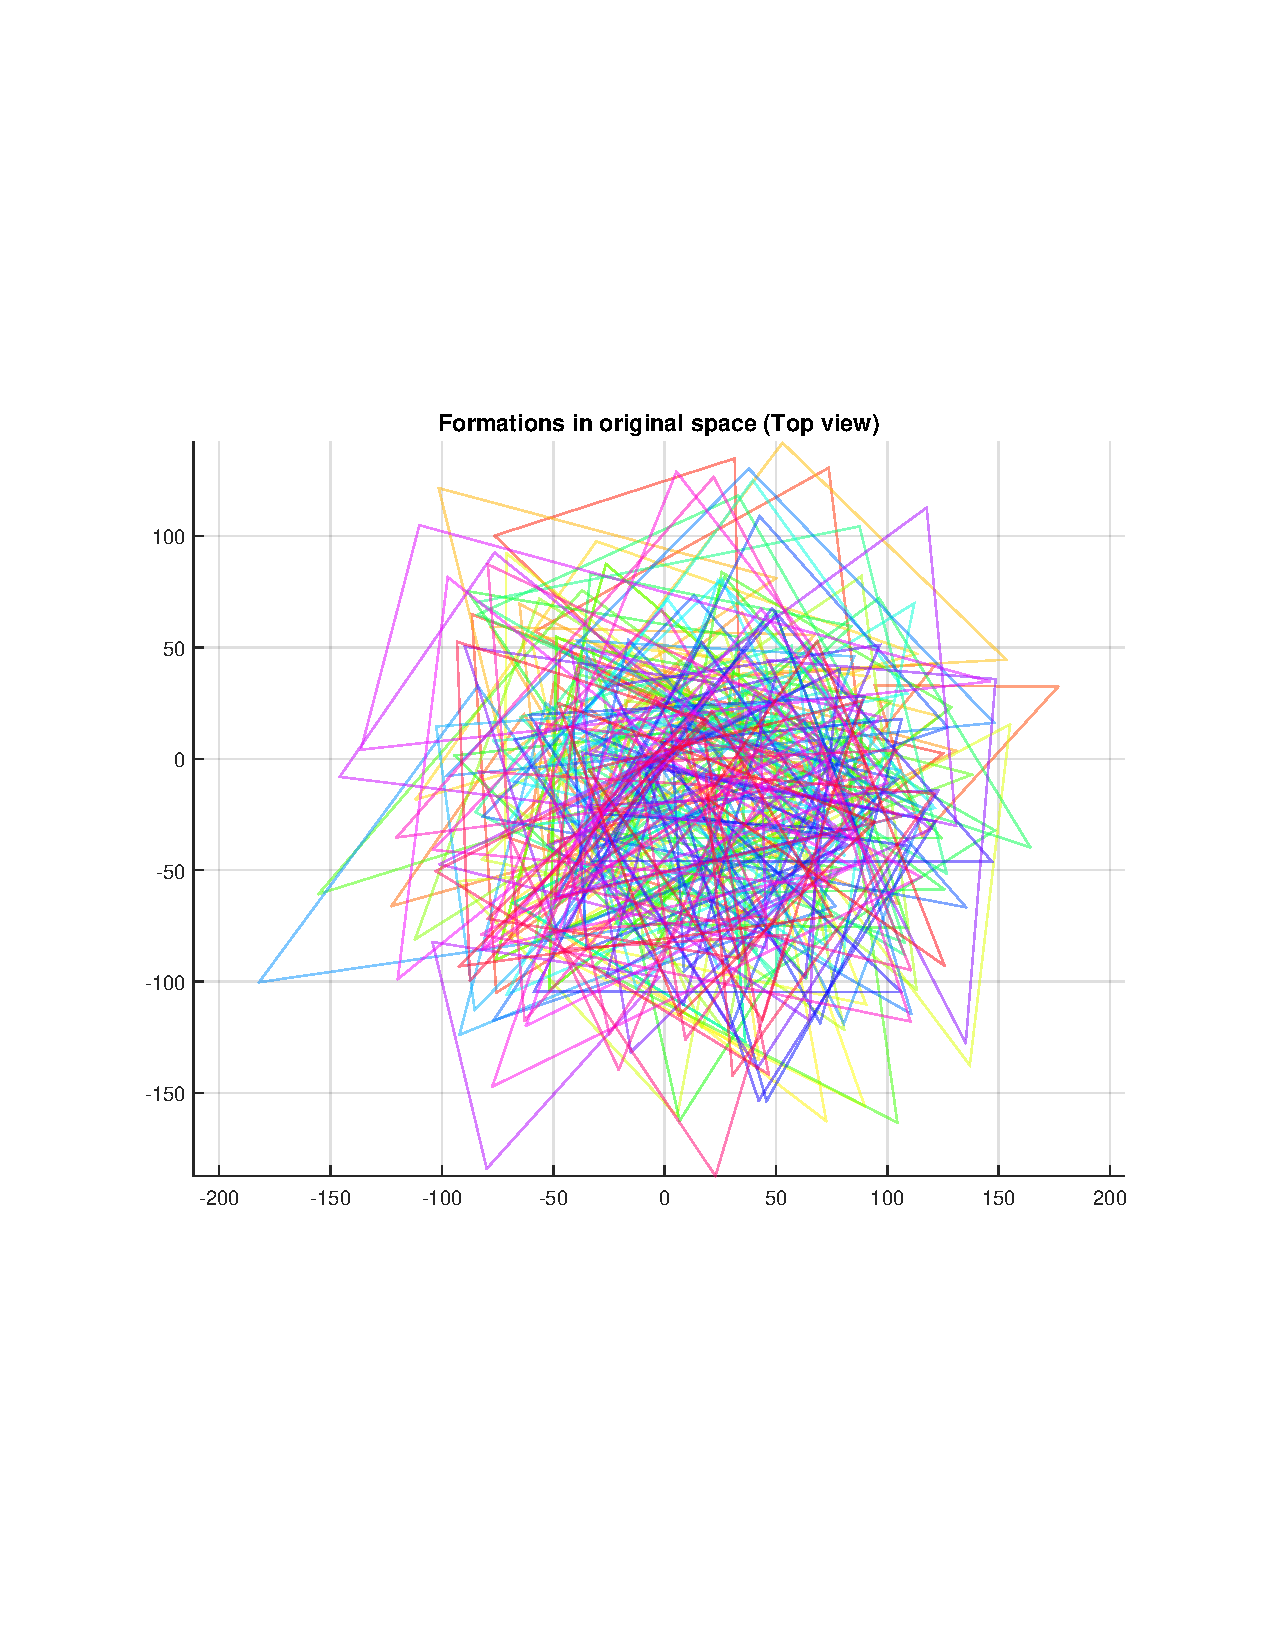
\includegraphics[trim=60 200 60 150,clip,width=0.32\linewidth]{figures/socialgeometry/originalTri}
	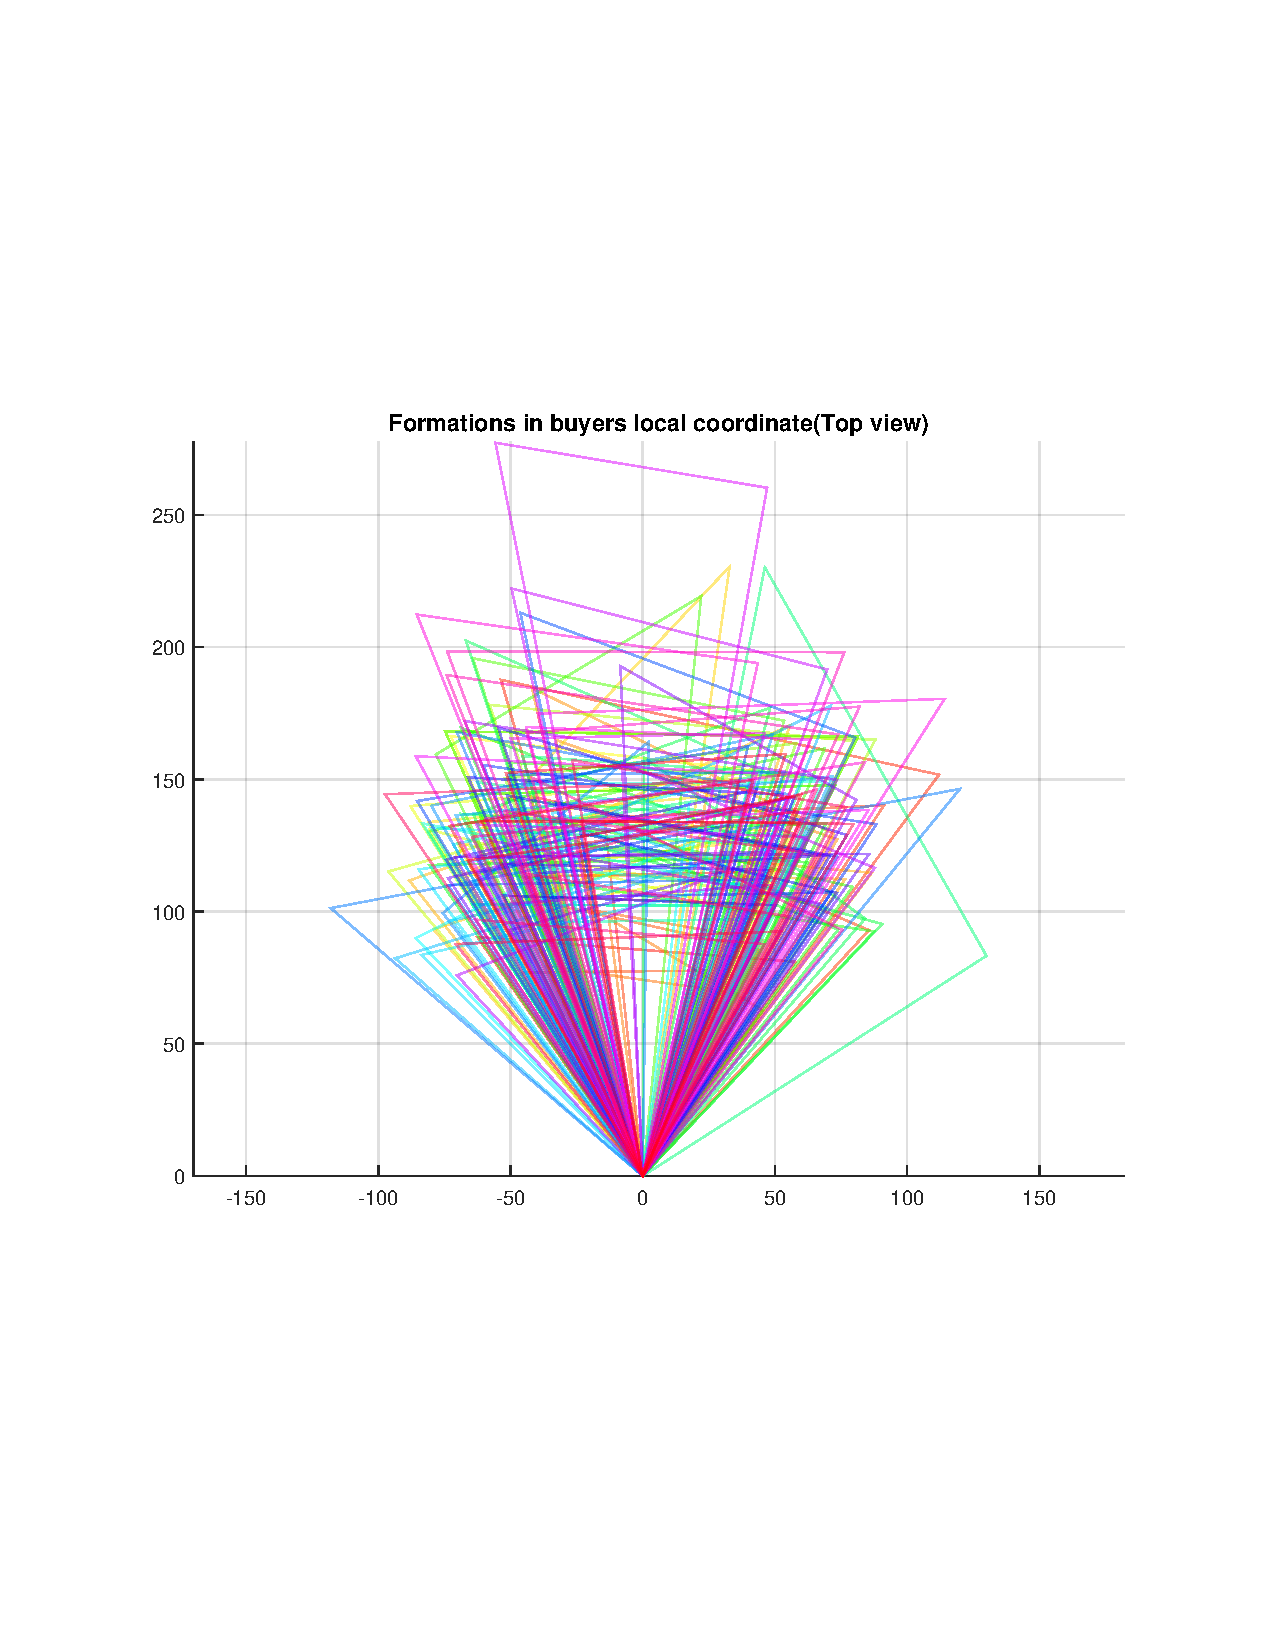
\includegraphics[trim=60 200 60 150,clip,width=0.32\linewidth]{figures/socialgeometry/buyersTri} 
	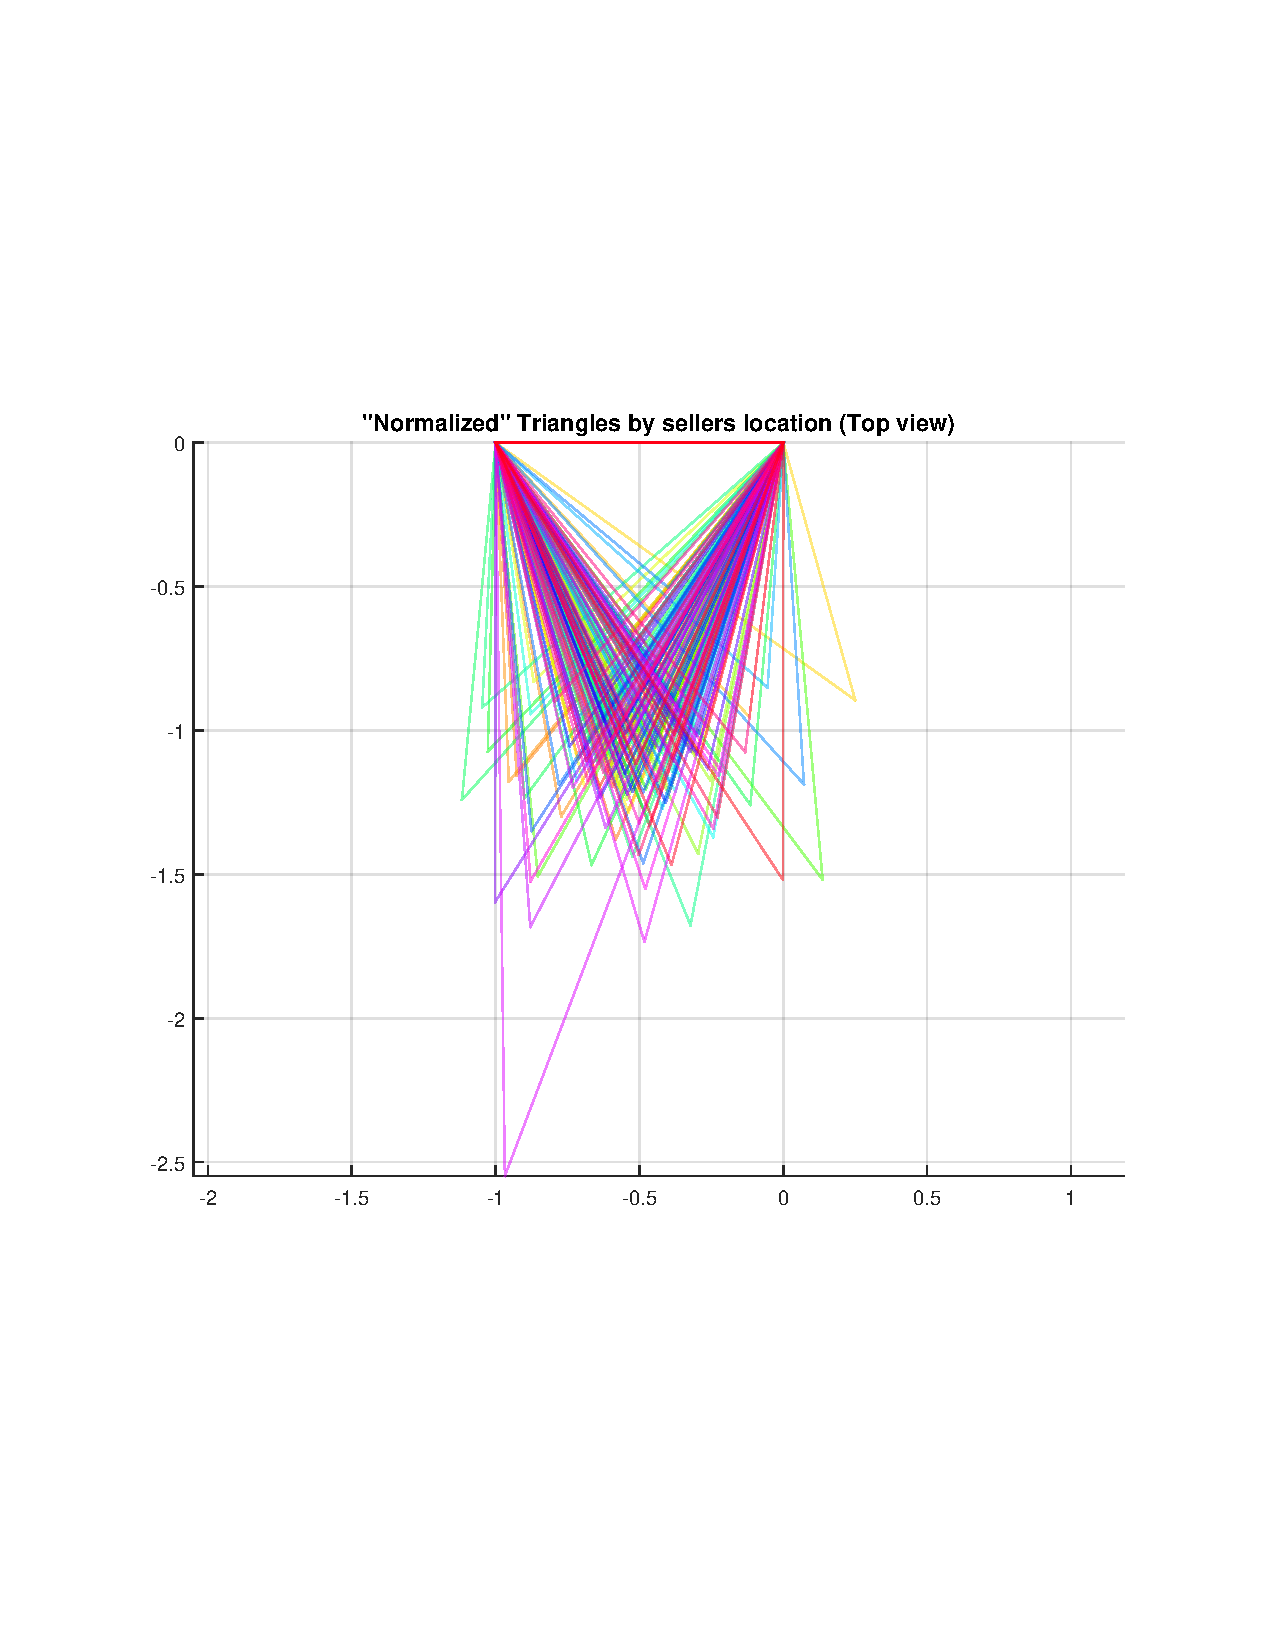
\includegraphics[trim=60 200 60 150,clip,width=0.32\linewidth]{figures/socialgeometry/normTri} 
	%	\subfigure[TrajCompares]{\label{Fig:asso_traj}\includegraphics[width=0.5\textwidth]{img/trajCompare}}   
	\caption{Social formations in three different representations. (a) Global coordinate; (2) Person-centric coordinate defined by buyers; (3) Normalized-by-a-pair coordinate system define by two sellers} 
	\label{fig:socialgeo_distribution}
\end{figure}

\section{Verification of Existing Theories: Proxemics}
Our large scale dataset measuring kinesic signals of interacting people enables to revisit existing well-known theories in psychology by providing hard measurements. In this thesis proposal, we revisit proxemics model~\cite{Hall66} by using 59 haggling sequences in our dataset\footnote{This is a subset of our dataset. The remaining parts are still in the middle of precessing for body motion reconstruction.}, and compare the location measurements in our dataset with the distance categories defined in \cite{Hall66}. To analyze the formation and distance among people we compute an average formation for each group. The results are shown in the Figure~\ref{fig:socialgeo_distribution} by using three different coordinate systems: (1) world coordinate;  (2) person centric coordinate by a buyer; and (3) normalized-by-a-pair coordinate by two sellers. The plots clearly show that the formation is often similar to isosceles triangles with relatively far distances between a buyer and two sellers than the distance between sellers.

Table~\ref{table:proxemics} shows the distance among people, and we found that the results follows the social distance categories defined in the Hall's categorization~\cite{Hall66}. The distances among sellers are within the close phase of social distance ranges (from 120-210 $cm$) in \cite{Hall66}, and the average distance among sellers and buyers are within the far phase of social distance (from 210 to 370 $cm$) in \cite{Hall66}. %Our measurement shows that the relation of people in our scenes belong to this category, which should be correct.


 %In particular, this is because of the nature of the game since the buyer mainly gains attentions from two sellers. 

\begin{table}[]
	\centering
	\caption{Average Distances between people}
	\label{table:proxemics}
	\begin{tabular}{l| l| l| l| l}
		\hline
		Types & Avg. dist. (cm) & Std.(cm) & Min dist. (cm)  & Max dist. (cm)\\
		\hline
		Buyer-LeftSeller & 148.14 & 30.09 & 77.46 & 234.47 \\
		\hline
		Buyer-RightSeller & 149.43 & 30.81 & 88.45  & 283.62 \\
		\hline
		LeftSeller-RightSeller& 119.56 & 22.87  & 67.90  & 242.15 
	\end{tabular}
\end{table}


%
%\section{Kinesic Geometry Prediction}
%%사람이 의사소통과정에서 특정한 거리나 formation을 갖춘다는것은 심리학자들 사이에서 오랫동안 알려져왔고 연구된 사항이다. Edward Hall 은 이분야의 pioneer로 social interaction 상에서 인간의 공간적인 사용습성을 measure하여 여러 단계의 range of distance로 구분하였다. Kendon은 사람의 의사소통과정에서 생기는 동심원 모양의 패턴에 대한 연구를 하였다. 몇몇 최근 computer vision 페이퍼에서도 이런 연구결과를 발전하여 f-formation을 자동으로 분석한다거나, 영상에서 사람의 3D orientation을 자동으로 측정하려는 시도가 있었고 이에 관련된 데이터셋도 등장했다. 이 섹션에서는 가장 간단한 레벨의 signal인 의사소통과정에서 사람의 ditance와 orientation에 대해 연구하고, 이것을 모델링 하여 기계가 예측하는 방법을 제안한다.
%
%As a way to understand social interaction, the objective our research is to regress a function$F$ to predict the output signal of the target person, given input signals. If the function produces the same output as ground truth value of the target person, we can conclude that the model learn how human interact using nonverbal signals. A Deep Neural Network is used as the model, and we try various social signal prediction given various input signals. To this end, we also quantify the importance of each channel of social signal for each type of social interaction task. In this study, we use the haggling sequences capture by 122 participants where each game is performed by three people following the game protocol. 
%
%We denote $\mathbf{P}_1$ to specify the target person we are interested in to predict, and two other people are denoted as $\mathbf{P}_l$ and $\mathbf{P}_r$, where $\mathbf{P}_l$  is on the left side than $\mathbf{P}_r$ in the person-centric view of $\mathbf{P}_1$. 

\begin{figure}[t]
	\centering
	\includegraphics[width=\textwidth]{figures/pred_gaze_ex}\\
	\includegraphics[width=0.32\textwidth]{figures/firstpersonview_1}
	\includegraphics[width=0.32\textwidth]{figures/firstpersonview_2}
	\includegraphics[width=0.32\textwidth]{figures/firstpersonview_3}
	\caption{We predict gaze direction of a target person (a buyer) in the haggling game sequences. The first row shows an example scene with measured signals including anatomical landmarks from body, face, and hands. The ground truth gaze direction is computed by computing the normal direction of a face. The second rows show artificial first person views from example scenes. This visualization enable us to illustrate the received signals of the target person during the interaction.} 
	\label{fig:gazepred_probdef}
\end{figure}

\section{Kinesic Signal Prediction: Predicting Attention}
In this thesis proposal, we present a method to predict attention signals of an individual in triadic social situations (Haggling games in our dataset). The objective of this task is to predict facial orientation (gaze direction or attention) of a target person $\mathbf{P}_1$, given body motions of other two people, $\mathbf{P}_2$ and $\mathbf{P}_3$. In a social interaction, a person tends to pay attention to a single person at each time, and the motivation of this task is to study what type of kinesic signals attract attentions from others in social communication.

We represent the gaze direction of the target person $\mathbf{P}_1$ in the normalized-by-a-pair coordinate system defined by $\mathbf{P}_2$ and $\mathbf{P}_3$ (we assume that $\mathbf{P}_2$ is on the left than $\mathbf{P}_3$ in the person centric coordinate system of $\mathbf{P}_1$, as shown in Figure~\ref{fig:ssp_notation1} (d)), where $\hat{\theta}_1^{2,3}=0$ when the target person faces $\mathbf{P}_3$ and $\hat{\theta}_1^{2,3}=1$ in the opposite case. An example scene of a haggling sequence is shown in Figure~\ref{fig:gazepred_probdef}.

Formally, we regress the function $F_1$ by an optimization:
\begin{align}
\mathbf{O}_1(t) = \operatorname{F}_1 \left( \mathbf{I}_1  (t) \right),
\end{align}
where $\mathbf{O}_1(t) = \{ \hat{\theta}^{2,3}_1 \}$ and $\mathbf{I}_1(t) = \{ \mathbf{B}_2, \mathbf{B}_3 \}$. Intuitively, this function takes other people's body postures at a single time as input and predicts the attention direction of the target person. This prediction problem enables us to study how people use their body parts to attract attention from others in their turns. In this thesis proposal, we only consider a body posture at a time instance as a simple case, but plan to consider various combination of signals including motions in a range of time as input for the function. 

We use Deep Neural Network (DNN) to define the regression function $F_1$. To simplify the problem we quantize the ground truth value into $\hat{\theta}^{2,3} = \{0,1\}$ using a threshold $0.5$, and train the model as a binary classification problem. We found that a simple feed forward network with three layers works reasonably well in this task.
%
%\begin{figure}[t]
%	\centering
%	\includegraphics[width=0.3\textwidth]{figures/firstpersonview_1}
%	\includegraphics[width=0.3\textwidth]{figures/firstpersonview_2}
%	\includegraphics[width=0.3\textwidth]{figures/firstpersonview_3}
%	\caption{Social communication between a sender and a receiver} 
%	\label{fig:firstpersonview_1}
%\end{figure}

%Network graph
%Other option is to use a sequence of previous signals to predict current motion. As another objective, we may consider a series of future output signals (seq2seq). 

\begin{figure}[t]
	\centering
	\includegraphics[width=\textwidth]{figures/model4_static}
	\caption{Gaze prediction accuracy for combinations of of kinesic signals. The first row is the results by using the target person's body signals, and the results on the second row are by using only the other two participants' signals.} 
	\label{fig:prediction_accuracy}
\end{figure}

\begin{figure}[h]
	\centering
	\includegraphics[width=\textwidth]{figures/gazepred_graph}
	\caption{A gaze prediction result for two example sequences (test sequence 8 and 10). For each example scene, the first row is the result by using the target person's body signals, and the second row is the result by using other two participants' signals.}
	\label{fig:gazepred_graph}
\end{figure}


\subsection{Experimental Results For Gaze Prediction}
In this section, we shows a preliminary experimental result on the attention prediction task. We use 59 haggling sequences, and only consider a buyer in each game as a target person, since their gaze directions tend to be correlated to sellers kinesic signals. We divide the dataset into 49 training set and 10 testing set. A feed forward network with 3 layers (the number of hidden units are 14,14,1 respectively) is used as the regression model, and we train the network using the cross entropy loss. 

The ground truth gaze direction of the target person is computed by finding a normal direction from face landmarks of the target person at each time instance. As input of the function $F$, we put body signals of others $\{ \mathbf{B}_2, \mathbf{B}_3 \}$, and also we perform additionally experiments by using only a subset of other people's body signals (e.g., using only the signals from wrist), or by using only the target person's own body signals $\{ \mathbf{B}_1\}$. 

The accuracy is shown in Figure~\ref{fig:prediction_accuracy}. The second row of the table shows the prediction performance by using other people's body signals as input. As can be seen, we found that signals from arms are more important than leg signals in predicting attentions, which means that arms have more distinctive features in attracting attention than legs. The accuracy of using arms is 67 percent, while the accuracy by using legs are about 60 percent. The best performance is obtained by observing all joint signals except legs, showing that legs are even distracting the attention prediction models. This results can be intuitively understood, since people tend to use their hands during their turns with speaking. The differences in accuracy can be considered as a quantification of signal influence of each body parts related to attracting attention in a social situation. For example, we may consider that heads are 3 percent more important than legs and wrists are about 6 percent more important than legs, in term of prediction accuracy. However, a better representation can be considered to provide more intuitive representation in terms of signal bandwidth, as a future goal.     

The result by using the target person's own signals is also shown in the first row of Figure~\ref{fig:prediction_accuracy}, and the result shows that the head posture of the target person is the most important part in predicting its own gaze direction, which is an reasonable conclusion because the ground truth gaze direction is computed from the head orientation. 

The attention prediction results at each time of two full example test sequences are shown in the  Figure~\ref{fig:gazepred_graph}, where all the body joints of target person and others are used for each graph. The qualitative results of attention prediction is also shown in  Figure~\ref{fig:gazepred_qualitative}.  This trained model is considered as an artificial agent which communicates with humans using its attention by accepting other people's kinesic signals, and we found that it already show its ``understanding" about how humans use their attentions and kinesic signals in a social situation.

\begin{figure}[t]
	\centering
	\includegraphics[width=\textwidth]{figures/gazepred_qualitative}
	\caption{Qualitative results in predicting attention direction of buyers in haggling sequences. The red arrows show the predicted gaze directions in a time instance.} 
	\label{fig:gazepred_qualitative}
\end{figure}


\pagebreak

%We compute the accuracy in binary classification using whole bodies with all the three people's body joints. The accuracy is 83 percent.  

%
%\subsection{Predicting Positions}
%%Given similar input, we can also predict the relative location of the target person from other two. 
%
%\subsection{Predicting Facial Expression}
%
%\subsection{Predicting Body Motion}
%Gaze direction is strongly related to body motion since it is a part of it. However, since we always fix other two people's motion, we expect that gaze is on either two. I need to check how it will look like in GT data, and also need to make a way to denormalize this. 

%\section{Overview}
%	The objective of \emph{Social Signal Prediction} is to forecast the future signals that the target person will transmit to transmit his/her information given all the signals up to the time that the target person takes into account consciously and unconsciously. 
%Let us assume that all types of signals emitted from a single target person at time $t$ are represented as $\mathbf{x} (t)$. Here, we define $\mathbf{x} (t)$ to include verbal signal, $\mathbf{x}_v (t)$,  nonverbal signals, $\mathbf{x}_n (t)$, and even non-measurable internal ``signals" of the person, $\mathbf{x}_{\omega} (t)$, such as feeling, emotions, thought, belief, religion, knowledge and so on, which can affect the future motion of the target person\footnote{Such non-measurable signals can only be ``measurable" by the target person oneself.}.
%\begin{equation}
%\mathbf{x} (t) = \{  \mathbf{x}_v (t), \mathbf{x}_n (t), \mathbf{x}_{\omega} (t) \}
%\end{equation}
%
%We also define the signals $\mathbf{y}(t)$ originated from outside and received (or sensed) by the target person. This signals contains verbal $\mathbf{y}_v (t)$ and non-verbal signals l $\mathbf{y}_n (t)$ by other people which the target person can sense, and also contains signals from all the non-human environment $\mathbf{y}_e (t)$ which affects the target person's future motion. As examples of the $\mathbf{y}_e (t)$, the existence of roads makes the person to walk on it, and existence of wall restricts the movements of target person. 
%\begin{equation}
%\mathbf{y} (t) = \{  \mathbf{y}_v (t), \mathbf{y}_n (t), \mathbf{y}_{e} (t) \}
%\end{equation}
%Note that $	\mathbf{y} (t)$ should be measurable by the target person's sensing system (otherwise the signals do not affect to the target person's future motion), and we ignore all the non-sensible signals (e.g., ultra sound). Also note that, in social communication scenarios, the target person receives signals by other people,  that is  $\{\mathbf{y}_v (t), \mathbf{y}_n (t) \} \neq \phi$, but, in non-social situation, this signal values are null and only $\mathbf{x}_{y} (t) \neq \phi$ (because environments are always there).
%
%
%In practice, humans use all the current and previous information to make a future decision. Similarly, Social Signal Prediction takes into account all the the transmitted and received singals up to the time to predict the future signals of the target person $\mathbf{x} (t+1)$. Formally, the goal is to regress a function $\mathcal{F}$ defined as:
%
%\begin{equation}
%\mathcal{F} \left( \mathbf{x}  (t_0:t),   \mathbf{y} (t_0:t) \right)   =\mathbf{x} (t+1),
%\label{equation:F}
%\end{equation}
%where $\mathbf{x}  (t_0:t)$ and $ \mathbf{y} (t_0:t)$ represent signals from time $t_0$ to $t$, and the $t_0$ denotes the very initial time that the target person transmits/receives any signals (basically his/her birth). Intuitively, $\mathcal{F}$ produce the right next future signals using all the previous inside-out and outside-in signals. $\mathcal{F}$ may produce the output by using near current time signals such as "nodding" as an reaction of somebody's "speaking" signals. $\mathcal{F}$  can govern all type of motion human commonly do without much thought. For example, it includes maintaining certain distance from other people, and facing each other during communications. The existence of  $\mathbf{y}_{e}\}$ in $\mathbf{y}\}$ is important because it will greatly affect future motion. For example, two pedestrians can talk each other without facing each other, because of the "road" signals in $\mathbf{y}_{e}\}$ and "walking" signals in $\mathbf{x}_{n}\}$ and $\mathbf{y}_{n}\}$. By using these source, we can predict the target person will still walk on the road. If the other person suddenly stops and look at the sky, this person's nonverbal signal $\mathbf{y}_n\}$ greatly affects the target person's motion, and we can predict the target person also stops and look at the similar direction. After that we may predict they will keep walking on the road since $\mathcal{F}$ knows that they were walking a while ago as input.
%
%Essentially, the Equation~\ref{equation:F} models human itself by observing all the input and output signals the person receive and transmit thorough life. Based on the signal the person is collecting the person's future prediction should vary, which reflect the person's culture, education, personality and so on. The core idea of our model is that it only uses measurable signals as input and output, and avoid to model the complicated conversion between internal messages to signals. 
%
%In practice, however, it is very infeasible to collect such data from the birth. So we restrict the scope so that the function only takes a short-term history of signals, by designing a special capture scenarios (a negotiation game). We hypothesize that by regressing the function \cite{equation:F} with lots of people, we can model human's behavior focusing on the short-term inputs by canceling out personal and cultural factors. In this paper we address the following objective function:
%\begin{equation}
%\mathcal{\tilde{F}} \left( \mathbf{\tilde{x}}  (t-w:t),   \mathbf{\tilde{y}} (t-w:t) \right)   =\mathbf{\tilde{x}} (t+1).
%\label{equation:F_ours}
%\end{equation}
%
%The function $\mathcal{\tilde{F}}$ takes input and output from the short-term history, from time $t-w$ to $t$. The $\mathbf{\tilde{x}}$ represents a subset of $\mathbf{x}$, in particular in this paper we only consider parts of nonverbal signal, that is $\mathbf{\tilde{x}} \subset \mathbf{x}_n$ and $\mathbf{\tilde{y}} \subset \mathbf{y}_n$. Obviously, modeling  $\mathcal{\tilde{F}}$ may lose meanings if $\mathbf{\tilde{x}}$ and $\mathbf{\tilde{y}}$ are too limited. For example, consider a handshaking scene between two people. Without having body gestures but only measuring locations, we do not have a clue why two people are suddenly approaching each other. It should be more obvious if we can measure the other person stretch hand approaching me. 
%
%More importantly we assume that the input of the Equation~\cite{equation:F} is not the raw data that humans senses using organisms but the output processed by human perception system. For example, we assume that $\mathbf{x}$ and $\mathbf{y}$ are social signals such as body or facial motions rather than raw video data, otherwise the Equation~\cite{equation:F} should consider whole computer vision problem together. 
%
%
%
%The scenes are captured by the state-of-the-art camera system introduce by Joo et al.~\cite{Joo-15}. This system captures interacting multiple people using 480 VGA cameras, 31 HD cameras, 10 RGB+D sensors, and multiple microphones. As output of the system, full body 3D skeletons and facial landmarks are obtained. 
%
%\textbf{3D Body Reconstruction}: For body reconstruction, we use the first stage of the method of Joo et al.~\cite{Joo-15}~\footnote{The second stage is not performed due to reduce computation time.}. As a modification, we use more recently developed 2D pose detector~\cite{cao2016realtime} that are trained with MS COCO Keypoint dataset~\cite{lin2014microsoft}. The generated output have 19 joints and includes eyes and ears, which makes it possible to estimate normal directions of faces as an approximation of gaze direction.
%
%
%\textbf{3D Face Reconstruction}: We additionally reconstruct 3D face landmarks by running a 2D face detector and triangulating them with RANSAC. To detect faces, we use 31 HD cameras synchronized with the VGA cameras in the system. We use a version of face detector based on the body pose detector~\cite{wei2016convolutional} but trained on face dataset~\cite{}. We found this is comparable to other 2D face landmark detectors~\cite{Torre15}. We use the already reconstructed 3D body position to find ROI to run the face detector, which also provide associations of detected faces across views. Each face lanmark, then, reconstructed by triangulation and RANSAC. Each reconstructed 3D face has 53 landmarks (159 dimensions) . To reduce the dimension, we perform PCA and only use 20 PCA dimensions to represent each 3D face.
%ted 60 sequences with 30 participants which is about an hour of data.
%%	
%\subsection{Tasks and Representation}
%We regress the function in Equation~\ref{equation:F_ours} using our dataset. The input is a chunk of time series data and we only predict a single frame. During the test time we can generate a series of prediction by recursively running the function by using the predicted output as seed. During the test we vary the input and output types and dimensions to demonstrate the impact of having additional signals in social prediction problem. 
%
%\subsubsection{Single person signal vs social signals}
%The simple version is not using any outside-in signals and depends on the target person's own previous signal. A simple cyclic motions such as walking and running (demonstrated in previous work) can be modeled by this. These motions can often be predictable using physics (velocity, acceleration, and so on). However, communications are not in this kind form in general. We act and react according to the communication context. We can assume that having more signals from other person can improve the prediction performance.  In this case, we only consider 2D location from the top view, the inputs and outputs are defined by the concatenation of location and orientations. 
%
%\begin{gather}	
%\mathbf{x(t-w:t)} = [\Delta \mathbf{x}^{i}_i(t) ; \Delta \theta_i(t) ] \\ \nonumber
%\mathbf{y(t-w:t)} = [\Delta \mathbf{y}^{i}_i(t) ; \Delta \theta_i(t) ] \\ \nonumber
%\mathbf{y(t+h)} 
%\end{gather}
%
%
%\subsubsection{Level of Signals}
%A simplest form is just considering the 2D location of the people from the view on the top. Previous work tracking pedestrians~\cite{Alahi_2016_CVPR} lies in this category. However, group discussion including our negotiation scenario doesn't have dominant location changes keeping a particular formation. There body movement is very subtle. As a study, we change the level of signals from simple position and orientation information to body joints and faces, and see how prediction performance varies.
%\begin{gather}	
%\mathbf{x(t-w:t)} = [\Delta \mathbf{x}^{i}_i(t) ; \Delta \theta_i(t) ; j_2(t) ;.... ;j_{15}(t) ] 
%\end{gather}
%
%The way to use other people's signal can significantly affect the performance of the prediction. We present multiple structure and see the performances. 
%
%The first case is don't care the global positing among people but just keep the information.
%\begin{gather}	
%\mathbf{y(t-w:t)} = [\Delta \mathbf{y}^{i}_i(t) ; \Delta \theta_i(t) ; j_2(t) ;.... ;j_{15}(t) ] 
%\end{gather}
%
%The next method is to use their spacial relations. 
%
%\begin{gather}	
%\mathbf{y(t-w:t)} = [\Delta \mathbf{y}^{j}_i(t) ; \Delta \theta_i(t) ; j_2(t) ;.... ;j_{15}(t) ] 
%\end{gather}
%
%Note that the location changes of y is in person centric coordinate of the target person. 
%%Intuition of this method
%
%\subsection{Predicting Social Signals: Methods}
%
%We perform the experiment using multiple baselines. 
%
%\subsubsection{Nearest Neighbor}
%As the simplest method, we implement nearest neighbor method to find the best prediction.
%
%\subsubsection{LSTM}	
%As another method, we use LSTM which most populary used in time series prediction problems. 
%
%\subsubsection{Wavenet}
%Recently, wavenet shows great performance on the audio data. We applied this method on our motion data. 
%
%
%
%\subsection{Results}
%
%We compare the performance of single person future motion prediction. 
%First we separate test set and training set from all available haggling sequence. And the test chunks in the testing set is generated by selecting $f$+1 frames ($f=100$ in our experiments), and sampling by shifting $w=5$ frames. 
%
%The prediction is performed only for a single subject both cases (independently vs group based). However, in the presented based based on group information, other people's signals are still used for the target subject's motion prediction.
%
%\subsubsection{Evaluation}
%How to evaluate the prediction results is not straightforward, since human can move with lots of variation. Without knowing all the singals, this cannot be feasible, and it will be worse in the long term prediction cases. In our paper, we simply compute RMS error from the measured ground truth data, and also compute PCK graph for further analysis. 
%
%\subsubsection{Social Formation Prediction}
%In this scenario, we only consider the location and orientation of each person. Given a person's location, we model how the location and orientation will be of the target person. 
%
%We compare diverse type of inputs and representations. The errors are computed in the original coordinate system to be fair. 
%
%1. Increasing dimension of X. Body only, Face, Face+ body 
%2. Presenting Increasing dimension of Y. Other peoples
%
%%
%%\begin{figure}[h]
%%	
%%	\includegraphics[trim=100 200 120 150, clip=true, width=0.18\textheight]{experiment/wavenet1/wavenet_representation_compare-RMS-error-(oriSpace,-locationOnly-only[=3]-)}
%%	\includegraphics[trim=100 200 120 150, clip=true, width=0.18\textheight]{experiment/wavenet1/wavenet_representation_compare-RMS-error-(oriSpace,-orientation-only[=1]-)}
%%\end{figure}
%

\clearpage

\pagebreak